\documentclass[a4paper,12pt,fontset=none,twoside]{article}
\usepackage{ctex}
\usepackage{ulem}
\usepackage{titletoc}
\usepackage{enumerate}
\usepackage{CJKulem}
\usepackage{times}
\usepackage{setspace}
\usepackage{indentfirst}
\usepackage{fancyhdr} 
\usepackage{graphicx}
\usepackage{amsmath}
\usepackage{amssymb}
\usepackage{booktabs}
\usepackage{array}
\usepackage{caption}
\usepackage{float}
\usepackage{multirow}
\usepackage{xunicode,xltxtra}
\usepackage{wrapfig}
\usepackage{fontspec}
\usepackage{subcaption}
\usepackage{minted}
\captionsetup[listing]{name=Code}


%\usepackage{subfigure}
\usepackage{nicematrix}
\usepackage{makecell}

\usepackage{titlesec}
\usepackage{tikz}
\usepackage{gbt7714}
\usepackage{bbm}
\usepackage[top=23mm,bottom=21mm,left=24mm,right=24mm]{geometry}
\setcitestyle{numbers,super,open={[},close={]}}
\setlength{\headheight}{15pt}
\raggedbottom
\XeTeXlinebreaklocale "zh"
\XeTeXlinebreakskip = 0pt plus 1pt minus 0.1pt
\usepackage{listings}
\usepackage[most]{tcolorbox}
\usepackage{color}
\definecolor{blue}{RGB}{42,61,208}
\definecolor{dkgreen}{rgb}{0,0.6,0}
\definecolor{gray}{rgb}{0.5,0.5,0.5}
\definecolor{mauve}{rgb}{0.58,0,0.82}
\definecolor{idlekvred}{RGB}{168,29,52}
\definecolor{codebg}{RGB}{248,249,250}
\definecolor{codeframe}{RGB}{218,223,230}
\definecolor{benchred}{RGB}{158,27,50}
\definecolor{benchteal}{RGB}{44,133,139}
\definecolor{benchdark}{RGB}{82,82,82}
\definecolor{benchline}{RGB}{124,124,124}
\definecolor{benchbg}{RGB}{247,247,247}
\usetikzlibrary{arrows.meta,backgrounds,fit,positioning}

\lstdefinestyle{idlecpp}{
	language=C++,
	basicstyle=\ttfamily\small,
	backgroundcolor=\color{benchbg},
	keywordstyle=\color{benchred}\bfseries,
	commentstyle=\color{benchline}\itshape,
	stringstyle=\color{benchred},
	identifierstyle=\color{benchdark},
	numberstyle=\sffamily\scriptsize\color{benchline},
	numbers=left,
	stepnumber=1,
	numbersep=10pt,
	showstringspaces=false,
	showspaces=false,
	showtabs=false,
	breaklines=true,
	breakatwhitespace=false,
	columns=fullflexible,
	keepspaces=true,
	tabsize=4,
	aboveskip=0pt,
	belowskip=0pt,
	morekeywords={true,false,nullptr},
	emph={async_read,process_input,async_write},
	emphstyle=\color{benchteal}
}

\newtcblisting{codebox}[2][]{%
	enhanced,
	listing only,
	breakable=false,
	colback=codebg,
	colframe=codeframe,
	boxrule=0.6pt,
	arc=2pt,
	left=4pt,
	right=4pt,
	top=4pt,
	bottom=4pt,
	title={#2},
	fonttitle=\bfseries,
	coltitle=black,
	listing options={style=idlecpp},
	#1
}

\numberwithin{figure}{section}
\numberwithin{equation}{section}
\numberwithin{table}{section}

\let\kaishu\relax
\let\songti\relax
\let\heiti\relax
\IfFontExistsTF{楷体}{
  \newCJKfontfamily\kaishu{楷体}[AutoFakeBold={2.5}]
}{
  \IfFontExistsTF{AR PL UKai CN}{
    \newCJKfontfamily\kaishu{AR PL UKai CN}[AutoFakeBold={2.5}]
  }{
    \newCJKfontfamily\kaishu{Noto Serif CJK SC}[AutoFakeBold={2.5}]
  }
}
\IfFontExistsTF{宋体}{
  \newCJKfontfamily\songti{宋体}[AutoFakeBold={2}]
}{
  \IfFontExistsTF{AR PL UMing CN}{
    \newCJKfontfamily\songti{AR PL UMing CN}[AutoFakeBold={2}]
  }{
    \newCJKfontfamily\songti{Noto Serif CJK SC}[AutoFakeBold={2}]
  }
}
\IfFontExistsTF{黑体}{
  \newCJKfontfamily\heiti{黑体}[AutoFakeBold={1}]
}{
  \IfFontExistsTF{Noto Sans CJK SC}{
    \newCJKfontfamily\heiti{Noto Sans CJK SC}[AutoFakeBold={1}]
  }{
    \newCJKfontfamily\heiti{Droid Sans Fallback}[AutoFakeBold={1}]
  }
}

\titleformat*{\section}{\zihao{-2}\heiti\centering}
\titlespacing*{\section}{0pt}{0.5\baselineskip}{0.5\baselineskip}

\titleformat*{\subsection}{\zihao{-3}\heiti}
\titlespacing*{\subsection}{0pt}{0.5\baselineskip}{0.5\baselineskip}

\titleformat*{\subsubsection}{\zihao{4}\heiti}
\titlespacing*{\subsubsection}{0pt}{0.5\baselineskip}{0.5\baselineskip}

\setlength{\parskip}{0pt}
\setlength{\parindent}{2em}

\IfFontExistsTF{Times New Roman}{
  \setmainfont{Times New Roman}
}{
  \setmainfont{Liberation Serif}
}

\IfFontExistsTF{Noto Serif CJK SC}{
  \setCJKmainfont{Noto Serif CJK SC}
}{
  \setCJKmainfont{AR PL UMing CN}
}
\IfFontExistsTF{Noto Sans CJK SC}{
  \setCJKsansfont{Noto Sans CJK SC}
}{
  \setCJKsansfont{Droid Sans Fallback}
}


\usepackage[breaklinks,colorlinks,linkcolor=black,citecolor=black,urlcolor=idlekvred]{hyperref}
% [colorlinks,linkcolor=red,citecolor=green]

\setcounter{tocdepth}{3}
\renewcommand{\contentsname}{\centerline{\zihao{-2} {目\quad 录} \vspace{-8mm}}}

\titlecontents{section}
[0pt]
{\vspace{.2\baselineskip}\bfseries}
{\contentslabel{1.2em}}
{\hspace{-1.2em}}
{\hspace{.5em}\titlerule*[10pt]{$\cdot$}\contentspage}


%   页眉页脚
\pagestyle{fancy}     
\fancyhf{} 
\fancyhead[CO]{\zihao{-5}{\songti 宁波大学信息科学与工程学院学院本科毕业设计（论文）\vspace{0.4ex}}}
\fancyhead[CE]{\zihao{-5}{\songti 基于可扩展基数树的键值内存数据库设计 \vspace{0.4ex}}}
\cfoot{\thepage}

\begin{document}
\ctexset{bibname=\centerline{\zihao{-2}{参考文献\vspace{-8mm}}}}

\begin{titlepage}
	\begin{center}
		
\includegraphics[width=11.18cm]{figure//nbu.pdf}\\
		\vspace{13mm}
		\textbf{\zihao{1}{\kaishu {本科毕业设计（论文）}}}\\[0.8cm]
		\vspace{7mm}
		\begin{spacing}{1.2}
			\zihao{-2}{\heiti{\textbf{题目：基于可扩展基数树的键值内存数据库设计}}}

			% \zihao{-2}{\heiti{\textbf{顺序多分类方法}}}
			\vspace{2mm}

			\zihao{-2}{\textbf{IdleKV: Design of a Key-Value In-Memory Database Based on Adaptive Radix Tree}}
		\end{spacing}
		\vspace{20mm}
		\setlength{\extrarowheight}{3mm}
		{\songti\zihao{-3}
			\begin{tabular}{rp{10.75cm}<{\centering}}
				{\makebox[4em][s]{学\qquad 院}} & \heiti 信息科学与工程学院  \\\cline{2-2}
				{\makebox[4em][s]{专\qquad 业}} & \heiti 计算机科学与技术    \\\cline{2-2}
				{\makebox[4em][s]{班\qquad 级}} & \heiti 22计算机科学与技术2班 \\\cline{2-2}
				{\makebox[4em][s]{学\qquad 号}} & \heiti 226000581           \\\cline{2-2}
				{\makebox[4em][s]{学生姓名}}    & \heiti 陈一波              \\\cline{2-2}
				{\makebox[4em][s]{指导教师}}    & \heiti 辛宇              \\\cline{2-2}
				{\makebox[4em][s]{完成日期}}    & \heiti 2026年05月3日              \\\cline{2-2}
			\end{tabular}
		}\\[2cm]
	\end{center}
\end{titlepage}

\newpage

\begin{center}
	~\\[1.9cm]
	\textbf{\zihao{1}{\kaishu {诚\quad 信\quad 承\quad 诺}}}
\end{center}
\begin{spacing}{1.9}
	\vspace{2em}
	\zihao{4}{我谨在此承诺：本人所写的毕业论文《基于可扩展基数树的键值内存数据库设计》的主体均系本人独立完成，没有抄袭行为，凡涉及其他作者的观点和材料，均作了注释，若有不实，后果由本人承担并愿接受校方的处分。}

	\vspace{1em}
	\rightline{\textbf{\zihao{-3}{\kaishu {承诺人（签名）: 陈一波}}}}
	%\rightline{\textbf{\zihao{-3}{\kaishu {承诺人（签名）:\qquad \qquad}}}}

	\rightline{\textbf{\zihao{-3}{\kaishu {2026 年 5 月 24 日 \qquad}}}}

	\thispagestyle{empty}
\end{spacing}

\newpage
\begin{spacing}{1.35}
	\thispagestyle{empty}
	\tableofcontents  %生成目录
	\setcounter{page}{0}
	\thispagestyle{empty}
\end{spacing}
\newpage

\begin{spacing}{1.5}
	\setlength{\parskip}{0pt}
	\setlength{\parindent}{2em}
	\pagenumbering{Roman}
	\begin{center}
		\zihao{-2}{{\heiti 题目：基于可扩展基数树的键值内存数据库设计}}
		\phantomsection
		\addcontentsline{toc}{section}{摘要}

		\vspace{8pt}
		\zihao{-2}{\heiti{摘\quad 要}}
	\end{center}

	{\kaishu }

	{\heiti 关键字}\quad {\kaishu 内存数据库；键值存储；可扩展基数树；NoSQL }

	\newpage

		\begin{center}
		\begin{spacing}{1.2}
			\zihao{-2}{\textbf{IdleKV: Design of a Key-Value In-Memory Database Based on Adaptive Radix Tree}}
		\end{spacing}
		\phantomsection
		\addcontentsline{toc}{section}{Abstract}

		\vspace{0.8em}
		\zihao{-2}{\textbf{Abstract}}
	\end{center}

		\begin{spacing}{1.5}
		
		\vspace{0.5em}

		\textbf{KEYWORDS}\quad In-Memory Database, Key-Value Stores, Adaptive Radix Tree, NoSQL

	\end{spacing}


	\newpage

	\section{绪论}
	\pagenumbering{arabic}
	\setcounter{page}{1}
	\subsection{选题背景与意义}
	随着主内存容量增长和成本下降，越来越多的数据管理系统开始将关键工作集乃至全部事务数据驻留在内存中，以减少磁盘访问带来的高延迟开销；在 OLAP 场景中，生产系统也常通过引入内存缓存或内存加速层来降低交互式查询延迟、提升查询性能。其中 Key-Value 内存数据库在高并发、低延迟的数据处理场景中得到广泛应用，如：缓存系统、实时推荐、流式计算以及 AI 基础设施等等\cite{In-memory-databases-The-foundation-of-real-time-AI-and-analytics}。

	然而 Redis 作为目前最广泛使用的键值型内存数据库，仍采用单线程的执行模型，这一设计源于早期内存键值存储系统被认为是 I/O 密集型服务，单线程已能够满足性能需求。但在当前多核 CPU 成为服务器标配、网络带宽逐步增加的背景下，Redis 服务想要利用一台服务器上的多核 CPU 处理指令，通常需要依赖集群分片，这无疑从而增加了部署与运维的复杂度。

	另一方面，键值数据库的应用场景并不局限于简单的点查和更新。在排行榜、区间检索、前缀匹配、流式状态管理和推荐系统等场景中，系统还需要同时支持按 key 精确定位和按顺序范围访问。传统的跳表或通用树结构虽然能够提供有序能力，但在主内存场景下往往存在指针跳转较多、缓存局部性较差的问题。可扩展基数树（Adaptive Radix Tree, ART）通过路径压缩和自适应节点布局，在保持有序遍历能力的同时提高了内存访问效率，因此成为主内存数据库中一种具有潜力的有序索引结构。
	
	在上述背景下，设计一种兼顾 Redis 协议兼容性、多核扩展能力与高效有序索引结构的主内存键值数据库具有重要的研究价值与工程意义。

	\subsection{相关研究}
	主内存数据库、轻量级并发控制和高效有序索引是本文的三个核心技术背景，本小节将详细介绍这些主题当前的研究现状。

	\subsubsection{主内存键值数据库}
	随着主内存容量持续增长，越来越多的键值存储系统开始以 DRAM 作为主要数据承载介质，重新审视传统数据库中由磁盘主导的系统设计。Ousterhout 等人提出的 RAMCloud 是较早的代表性工作之一，它主张将数据常驻内存、将磁盘主要作为备份介质，从而在集群环境中提供低延迟、高吞吐的存储服务\cite{The-Case-for-RAMClouds-Scalable-High-Performance-Storage-Entirely-in-DRAM}。这一方向表明，当磁盘 I/O 不再位于关键路径上时，数据布局、网络路径和并发执行模型会成为影响系统性能的核心因素。

	在单机高性能键值系统方向，相关研究进一步把优化重点转向了多核并行执行和缓存友好的内存访问。MemC3 通过紧凑哈希表、近似 LRU 的 CLOCK 淘汰策略以及乐观锁等工程优化，显著提升了 Memcached 的内存利用率与并发性能\cite{MemC3-Compact-and-Concurrent-MemCache-with-Dumber-Caching-and-Smarter-Hashing}。MICA 则从请求分发、网络收包、数据分区和并行访问等多个层面协同优化，在通用多核服务器上实现了极高的单机吞吐\cite{MICA-A-Holistic-Approach-to-Fast-In-Memory-Key-Value-Storage}。进一步地，FASTER 利用缓存友好的并发哈希索引与混合日志相结合的设计，优化了点查、更新与 read-modify-write 路径，体现了现代键值存储对高并发更新场景的关注\cite{FASTER-A-Concurrent-Key-Value-Store-with-In-Place-Updates}。

	总体来看，主内存键值数据库相关研究主要围绕“如何充分发挥内存介质优势”和“如何在多核平台上压缩每次请求的常数开销”两个方向展开。然而，这类系统大多以无序键值访问、点查与更新负载为主要优化目标，对于兼顾 Redis 兼容接口、多核扩展能力和有序范围访问的统一设计关注相对较少，这也构成了本文工作的切入点。
	\subsubsection{主内存事务与并发控制}
	事务作为数据库领域最核心的主题之一，相关研究已经非常成熟。为了在保证基础的 ACID 性质的前提下尽可能提高并发度，提出了非常多的并发控制机制，这些机制大致可以分为两类：1.悲观并发控制；2.乐观并发控制。
	
	悲观并发控制协议通常基于锁来实现。Two-Phase Locking (2PL)作为一种基础的锁并发控制协议，它可以保证可序列化的（Serializable）事务一致性模型，最早由 Jim Gray 在早期研究中奠定了 2PL 基本思想，后来由 Bernstein 和 Goodman 在其关于并发控制机制的综合研究中予以系统化\cite{Concurrency-Control-in-Distributed-Database-Systems}。在此基础上，为了在提高事务并发度的，Gray 等人进一步提出了多粒度锁\cite{Granularity-of-locks-in-a-shared-data-base}，引入了层次结构的意向锁，在保证可串行化的前提下，有效降低了粗粒度锁带来的并发受限问题。

	乐观并发控制协议通常假设事务的冲突很少发生，在真正发生冲突时会重启事务。David P. Reed 在 1978 提出了一种基于时间戳（T/O）的乐观并发控制协议\cite{NAMING-AND-SYNCHRONIZATION-IN-A-DECENTRALIZED-COMPUTER-SYSTEM}，在单个事务涉及数据不多且冲突较少时，可以节省 2PL 中控制锁的额外成本，提高事务并发度。H. T. Kung 和 John T. Robinson 等人提出在此基础上提出一种更通用的乐观并发控制（Optimistic Concurrency Control, OCC）模型\cite{On-optimistic-methods-for-concurrency-control}，将事务执行过程划分为读阶段、验证阶段和写阶段，通过延迟冲突检测来提高系统的并发度与执行效率。

	传统并发控制协议起源于磁盘数据库时代，其设计目标主要围绕降低磁盘 I/O 开销与提升事务吞吐能力，因此系统瓶颈通常集中于存储访问延迟，并发控制开销相对次要。在主内存数据库中，数据完全驻留于内存，磁盘 I/O 不再构成主要瓶颈，并发控制机制的开销逐渐成为性能关键限制。针对上述问题，Kun Ren 等人提出一种轻量级的锁控制机制（Very Lightweight Locking，VLL）\cite{VLL}，通过去除中心化的共享/独占计数器与有序事务队列来推进可执行事务，以降低并发控制本身的元数据成本，使其在单核以及多核环境下都有非常优秀的性能表现。

	\subsubsection{可扩展基数树与有序索引}
	在有序索引方向，主内存场景的核心问题是如何在支持范围查询的同时减少树高、字符串比较与随机内存访问。Mao 等人提出的 Masstree 是这一方向的代表性工作，它将 trie 与 B\textsuperscript{+}-tree 拼接起来处理变长键与长公共前缀，并结合缓存友好的节点布局与细粒度并发控制，在多核主内存环境下兼顾了范围访问能力和较高吞吐\cite{Cache-Craftiness-for-Fast-Multicore-Key-Value-Storage}。这说明主内存环境下的有序索引设计，不能简单沿用面向磁盘的树结构，而需要显式考虑缓存层次和 CPU 访存成本。

	在此基础上，Leis 等人提出可扩展基数树（Adaptive Radix Tree, ART），通过路径压缩和 Node4、Node16、Node48、Node256 的自适应节点布局，在空间利用率和缓存局部性之间取得了更好的平衡\cite{The-adaptive-radix-tree-ARTful-indexing-for-main-memory-databases}。ART 的点查性能接近哈希索引，同时仍然保留了按字典序遍历、前缀匹配和范围扫描等有序能力，因此成为主内存数据库中非常有代表性的有序索引结构。

	不过，原始 ART 的设计重点主要在 key 上的有序访问，对于 Redis Sorted Set 这类需要按 score/member 复合顺序组织，并支持按 rank 定位和区间扫描的场景，并没有直接给出完整支持。因此，在将 ART 用于键值数据库有序容器时，通常还需要结合复合编码、迭代器和子树计数等机制进行扩展。也正因为如此，ART 既为本文提供了一个缓存友好的有序索引基础，也为进一步面向 Redis 语义做工程化增强留下了空间。
	
	\section{系统概述}
	本章主要概述 IdleKV 的整体设计原则与系统架构。描述系统中的核心模块（\allowbreak\texttt{Server}、\texttt{EventLoopPool}、\texttt{RedisService}、\texttt{IdleEngine}、\texttt{Transaction}、\texttt{Shard}、\texttt{DB} 以及 \texttt{Value}/\texttt{ZSet} 等数据结构）的主要职责及设计思路。

	\subsection{系统设计原则}

	\subsubsection{一致性保证}

	Redis 之所以能够在工程上较容易地提供强一致的可观察行为，一个重要原因在于其核心命令执行路径基本是串行化的。作为面向 Redis 语义的多核替代系统，IdleKV 不能只追求吞吐提升，还需要在并发访问场景下维持与 Redis 接近的事务可见性。因此，本文将 Strict Serializability 作为系统的一致性目标\cite{Linearizability:a-correctness-condition-for-concurrent-objects}，要求每个成功提交的操作既满足可串行化，又满足与真实时间顺序一致。

	本文使用 Elle\cite{Elle} 作为黑箱事务一致性检查器，对 IdleKV 生成的事务历史进行离线校验，用于验证当前实现是否满足预期的一致性模型。

	\subsubsection{Redis 协议兼容性}

	系统对外需要尽可能保持 Redis 风格的访问接口，使现有客户端、基准测试工具和运维脚本能够低成本迁移。为此，IdleKV 选择以 Redis Serialization Protocol（RESP）作为唯一网络交互协议，并尽量保持命令参数组织方式、返回值类型以及错误语义与 Redis 一致，从而降低系统替换与实验对比的门槛。

	考虑到论文原型实现的范围，初版系统优先支持 RESP2，并围绕字符串命令、基础系统命令以及 Sorted Set 相关命令构建完整处理链路。这样的取舍既能够覆盖本文关注的核心工作负载，也为后续继续补齐更完整的 Redis 命令集留下了清晰扩展接口。

	\subsubsection{垂直扩展性}

	垂直扩展性是本文系统设计的核心原则之一。与依赖集群分片提升吞吐的方案不同，面向单机多核的键值数据库应尽量减少共享状态与跨核通信开销，使请求尽可能在局部执行上下文中完成。为此，系统遵循“数据局部化、执行局部化、协调最小化”的设计原则：尽量将同一 key 的访问固定在局部处理单元中，避免热路径上的全局锁、频繁线程切换与不必要的同步操作，仅在必要时引入有限的跨核协作，从而在保证 Redis 兼容语义的前提下提升单机多核扩展能力。

	\subsection{系统总体架构}

	传统多线程系统通常依赖锁机制或原子操作来实现并发控制，然而，随着线程数量的增加，资源竞争显著加剧，导致系统性能难以随着 CPU 核心数的增长实现线性扩展。为此，IdleKV 采用 Shared-Nothing\cite{The-Case-for-Shared-Nothing} 架构，将系统划分为 $N$ 个相互独立的分片，其中 $N \leq$ CPU 核心数。每个分片由单一线程独占访问，并通过线程与 CPU 核心的绑定（CPU pinning）减少线程迁移带来的缓存失效开销。在该设计中，每个线程同时负责 TCP 连接处理以及对应数据库分片的管理，从而避免跨线程的数据访问与同步开销。
	
	在每个线程之上，IdleKV 采用更轻量级的 Fiber（协程）来执行不同的任务（如：数据操作执行、客户端连接处理以及异步 IO 等）。相比于操作系统线程，Fiber 具有更低的创建与上下文切换开销，其调度完全由用户态控制，从而避免了内核调度带来的额外开销。此外 IdleKV 能够根据系统特性设计调度策略，以此来提升线程内部的执行效率，增强系统在高负载场景下的可控性。详细内容将在第~\ref{sec:io-thread-model}章展开。

	\begin{figure}[htbp]
		\centering
		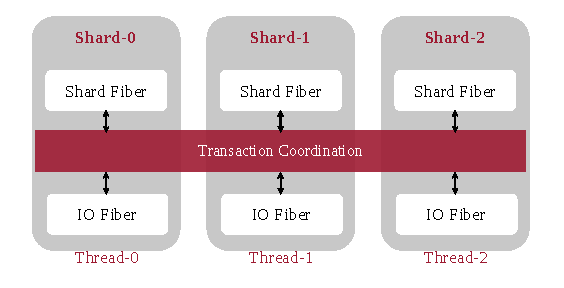
\includegraphics[width=0.95\textwidth]{figure/idlekv-architecture.pdf}
		\caption{IdleKV 整体架构图}
		\label{fig:overall-architecture}
	\end{figure}
	如图~\ref{fig:overall-architecture} 所示，IdleKV 在示例配置中创建了 3 个工作线程，每个线程独立负责其分片内的 I/O 处理与数据管理。当新的客户端连接到达时，系统会将对应的客户端协程（fiber）分配至某一线程执行。线程选择由调度策略决定，默认采用 Round-Robin（轮询）方式以实现负载均衡。在 Linux 环境下，若配置了 RPS（Receive Packet Steering），IdleKV 可进一步将连接调度至处理该网络数据包的 CPU 所对应的线程，从而提升 CPU 缓存局部性，优化整体性能。

	客户端的命令可能涉及到不同分片的数据，要保证多分片操作执行的全局顺序一致，就需要经过事务协调后，才能调度到对应分片的线程上执行数据操作。这里事务协调基于 VLL\cite{VLL} 并发控制机制来实现事务的全局顺序一致性，详细内容将在第~\ref{sec:vll-txn} 章中展开。

	\subsection{Redis Serialization Protocol 实现}

		RESP 是一种支持多种数据类型的二进制序列化协议,其控制序列使用标准 ASCII 编码。在 RESP 中，数据的第一个字节决定了其类型。当前 IdleKV 实现了 RESP2 中覆盖命令解析与结果返回所需的主要数据类型，其支持范围如表~\ref{tab:resp2-types} 所示。

		\begin{table}[htbp]
			\centering
			\small
			\caption{IdleKV 当前支持的 RESP2 数据类型}
			\label{tab:resp2-types}
			\begin{tabular}{p{3.0cm}p{2.2cm}p{2.6cm}p{6.2cm}}
				\toprule
				数据类型 & 前缀/形式 & 支持位置 \\
				\midrule
				Simple String & + & 响应 \\
				Error & \texttt{-} & 响应  \\
				Integer & \texttt{:} & 响应  \\
				Bulk String & \texttt{\$<len>}  \\
				Array & \texttt{*<len>} & 请求、响应  \\
				Null Bulk String & \texttt{\$-1} & 响应 \\
				\bottomrule
			\end{tabular}
		\end{table}


	IdleKV 同 Redis 相同，使用 RESP 作为 request-response 请求-响应协议，其工作方式如下：

	1. 客户端以“批量字符串数组”（array of bulk strings）的形式向 Redis 服务器发送命令。其中，第一个字符串表示命令名称，其后的元素则作为该命令的参数。

	2. 服务器则以 RESP 格式返回响应，响应的数据类型由具体命令的实现决定。
	
	IdleKV 实现了高效的 Zero Copy 的 RESP 协议 \texttt{Parser} 以及 \texttt{Sender}。
	
	首先是命令解析使用的 \texttt{Parser}，对于协议的数据类型、字符串长度和数组长度这样的头部数据，\texttt{Parser} 使用一个固定大小的缓冲区来处理，避免频繁的小内存分配，对于命令以及参数这样的数据本身，会被直接读取到一个已经提前申请好空间的 \texttt{CmdArgs} 类型中，在后续的所有操作中不会对 \texttt{CmdArgs} 中的参数做任何的移动以及拷贝。
	
	之后是用于响应恢复的 \texttt{Sender}，我希望尽可能减少 \allowbreak\texttt{write} 系统调用的次数，尽可能批量的发送响应，以此提高整个系统的吞吐，因此 \texttt{Sender} 内部有一个可扩容的写缓冲区，只有当缓冲区写满以及显示调用 \texttt{Flush} 时才调用 \texttt{write} 发送响应数据，这个对吞吐的提升是显而易见的，在实现过程中添加此优化后系统吞吐有 2$\sim$3 倍的提升。
	
	然而，对于 \texttt{GET}、\texttt{MGET} 等读操作而言，若将返回的 Value 数据拷贝至缓冲区再统一发送，会引入一次额外且可避免的内存拷贝。为此，\texttt{Sender} 在处理此类请求时仅持有 Value 数据的内存地址，而不将其复制至内部缓冲区。在实际发送阶段，采用 \texttt{writev} 系统调用将多个非连续内存区域（如协议头部与 Value 数据）组织为一组 \texttt{iovec} 结构进行聚合写入，从而在避免额外拷贝的同时，仍然保持批量发送的优势。此外，\texttt{Sender} 在持有 Value 内存引用期间，需要保证其生命周期的有效性。IdleKV 中 Value 采用 \texttt{std::shared\_ptr} 进行管理，因此 \texttt{Sender} 仅需持有一份指针拷贝，即可确保其在发送完成前不会被提前释放。
	

	\subsection{核心模块划分}

	IdleKV 中的核心模块还需要分章节展开详细说明，主要是如下三个部分：

	1. \textbf{基础设施}：为 Shared-Nothing 架构提供底层运行时支持，包括线程管理、网络 I/O、多路复用机制以及 Fiber 调度与同步原语等。

	2. \textbf{VLL 事务框架}：系统实现 Strict Serializability 一致性语义的核心模块，通过全局顺序控制与冲突管理机制，保证事务执行结果等价于某一全局串行顺序。

	3. \textbf{底层 DB 数据结构}：负责各类数据结构的具体实现，包括 KV 存储（KvStore）、有序集合（ZSet）等。

	\section{IO 与线程模型}\label{sec:io-thread-model}

	IdleKV 采用“线程级并行 + 线程内异步”的总体线程模型。系统通过多个工作线程利用多核 CPU 的并行能力，而在每个线程内部，则借助 Fiber 与事件循环实现 Proactor 风格的异步 IO 模式。需要特别说明的是，异步性（asynchronicity）与并行性（parallelism）并不等价：前者强调单个线程在等待 I/O 时不被阻塞，后者强调多个 CPU 核同时推进不同任务。IdleKV 同时利用了二者，即跨线程实现并行，在线程内部实现异步。

	在这一模型下，连接处理、分片任务执行等待任务都与一个 Fiber 绑定，Fiber 间采用主动让权的协调式 CPU 调度机制，Fiber 在遇到阻塞任务时或在一些条件下（如：到达 CPU 使用配额上限）就会主动放弃 CPU，由同线程中的其他 ready Fiber 继续运行。

	\subsection{基于 Fiber 的异步 IO}
	
	IdleKV 选择了 Boost.Asio 以及 Boost.Fiber\cite{Boost-Asio,Boost-Fiber} 来为系统提供异步 IO 以及协程调度的能力。Boost.Asio 在调用异步操作时需要传入的 completion token 来生成对应的 async handler（在异步任务完成时执行后需要执行的任务）以及 async result（异步操作的返回值操作）。通常 async handler 是一个回调函数，但逻辑复杂时会出现回调函数过多，核心逻辑混乱的问题，也不能和 Boost.Fiber 很优雅的结合在一起。

	为此，IdleKV 扩展了一种新的 completion token： \texttt{yield\_t}，并实现了 \allowbreak\texttt{yield\_handler} 负责将 fiber 挂起与唤醒。同时，还扩展实现了 \allowbreak\texttt{async\_result} 来返回异步操作的结果，把 fiber 的挂起与唤醒操作嵌入到异步流程之中，使异步代码能够以接近同步代码的方式书写如 Code~\ref{lst:yield-sync-io} 所示。

\begin{listing}[htbp]
\centering
\begin{minipage}{0.72\textwidth}
\begin{lstlisting}[style=idlecpp]
while (true) {
    nread = async_read(socket, buf, yield);
    res = process_input(buf, nread);
    nwrite = async_write(socket, res, yield);
}
\end{lstlisting}
\end{minipage}
\caption{使用 \texttt{yield\_t} 的同步风格 I/O 示例}
\label{lst:yield-sync-io}
\end{listing}

	从代码表面上看，上述逻辑与阻塞式 socket 编程非常接近；但实际上，当执行流到达 \texttt{async\_read()} 和 \texttt{async\_write()} 时，异步操作流程就如图~\ref{fig:asio-yield-flow} 所示。

		\begin{figure}[htbp]
			\centering
			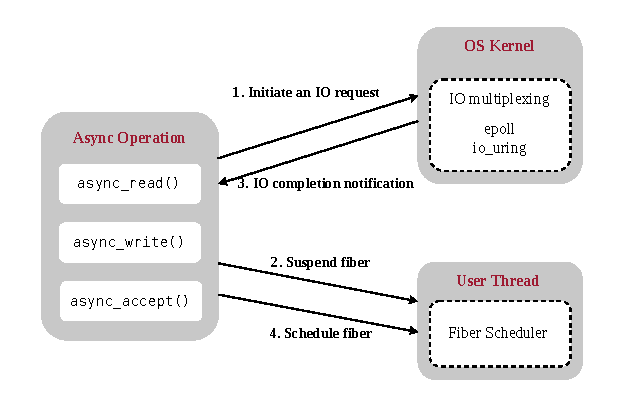
\includegraphics[width=0.60\textwidth]{figure/asio.drawio.pdf}
			\caption{基于 Fiber 的异步工作流程}
			\label{fig:asio-yield-flow}
		\end{figure}

	1. 注册 IO 请求；
	2. 挂起协程；
	3. IO 完成；
	4. 唤 醒 fiber 继续执行。

	\subsection{Fiber 调度机制}

	同一个线程上会允许各种各样的类型的任务，如：客户端请求处理、分片任务队列。为了最小化客户端的响应延迟，当一个客户端对一个分片发起读写请求时，我们希望尽可能快的执行对应操作。为此系统在事件循环线程中启用自定义优先级调度器，并为 Fiber 定义 HIGH、NORMAL 和 BACKGROUND 三个优先级，使 shard 任务队列消费者、连接处理和后台任务能够在同一线程内获得不同调度权重。

	仅有优先级还不足以保证线程内公平性。协调式调度的一个风险在于：如果某个 Fiber 长时间不主动让出 CPU，那么即使线程内部仍有其他 ready Fiber，也无法及时获得执行机会。为此，IdleKV 利用硬件 cycle counter 为热路径设置 CPU 预算，并在超过预算后触发主动 \texttt{yield}。其中，解析阶段和 Pipeline 聚合阶段分别由 \texttt{kMaxParseCpuCycles} 与 \texttt{kMaxSquashCpuCycles} 两个阈值约束，从而缓解单个长任务对线程内尾延迟的拖累。



	\subsection{Shared-Nothing 线程模型}

	IdleKV 的扩展性首先来自基于 key 哈希的 Shared-Nothing 分片模型，但系统并非只依赖“分片内串行执行”来保证一致性。
	
	
	\section{基于 VLL 的事务框架设计}\label{sec:vll-txn}
	IdleKV 在 Shared-Nothing 分片模型之上实现了一套基于 VLL 思想的事务框架。该框架的核心不是构建全局中心化锁管理器，而是让事务在进入执行前完成读写集分析，在每个目标 shard 上利用轻量锁表判断冲突、利用按事务号排序的 \texttt{TxnQueue} 维持局部顺序，并通过 \texttt{PollTransaction()} 推进当前可运行的事务。这样既保留了分片本地执行的缓存友好性，也使多 key、跨 shard 命令能够在统一抽象下获得确定的执行顺序。

	\subsection{Shared-Nothing 分片执行基础}
	IdleKV 的扩展性首先来自基于 key 哈希的 Shared-Nothing 分片模型，但系统并非只依赖“分片内串行执行”来保证一致性。对于单 key 命令，路由后通常只触达一个 shard；对于 \texttt{MGET}、\texttt{MSET}、\texttt{DEL} 等跨 key 命令，系统还会在各目标 shard 上执行事务注册、锁获取和顺序推进。因此，Shared-Nothing 提供的是第一层隔离边界，而基于 VLL 的事务框架负责补齐跨 shard 的执行次序与冲突控制，具体事务协调过程将在第~\ref{sec:vll-txn}章中展开。

	系统使用 \texttt{XXH64} 对 key 进行哈希，并从同一个 64 位哈希值同时得到 \texttt{ShardId} 和 key 指纹。前者决定命令应路由到哪个 shard，后者作为锁表索引参与后续的共享/独占冲突检测。每个 shard 维护多个逻辑数据库实例，对应 Redis 的 \texttt{SELECT} 语义。这样的设计把“数据归属”和“事务锁定”统一建立在同一套 key 预处理结果之上，减少了执行阶段的重复计算。

	每个 shard 内部都有一个有界任务队列，由高优先级 Fiber 负责消费。普通单分片命令可以直接作为任务提交到该队列执行；需要事务排序的命令则先在分片本地 \texttt{LockTable} 和 \texttt{TxnQueue} 中完成注册，再由 \texttt{PollTransaction()} 推进真正可运行的事务。换言之，任务队列负责把工作带到正确的 shard，而事务队列则负责在 shard 内维持符合事务号顺序的执行语义。与此同时，每个 shard 还拥有独立的 \texttt{ShardMemoryResource} 和 mimalloc heap，用于跟踪当前内存占用和峰值内存占用。事务对象虽然通过线程局部对象池复用，但 \texttt{Value}、\texttt{ZSet} 和 ART 节点等数据仍主要由所属 shard 的内存资源分配。这样既减少了跨线程分配器竞争，也使性能分析和资源统计能够自然落到 shard 粒度。

	\subsection{VLL 的核心思想与适用性}
	VLL 关注的核心问题是：在主内存数据库中，真正拖慢系统的往往不是用户逻辑，而是并发控制元数据本身。IdleKV 采用的事务框架并未机械复刻论文中的全部细节，而是吸收了其中最适合键值场景的三个要点，即轻量锁状态、事务入口排序和尽量局部执行。

	\subsubsection{轻量化锁管理的动机}
	VLL 的第一个启发是，锁对象不必设计成重量级结构。IdleKV 在每个 \texttt{DB} 内维护独立的 \texttt{LockTable}，每个锁槽只记录共享和独占两个计数器。事务注册时，写集合上的 key 指纹尝试获取独占锁，读集合上的 key 指纹尝试获取共享锁；如果检测到冲突，事务并不会立即执行，而是被标记为 \texttt{Blocked}。这种设计避免了围绕单条记录维护复杂的等待链表，把元数据开销压缩到了“哈希定位 + 计数器更新”这一较小范围内。

	\subsubsection{事务顺序与局部执行}
	VLL 的第二个启发是，事务顺序应尽可能在入口阶段确定。IdleKV 在命令解析后立即构造 \texttt{WRSet}，并通过 \texttt{InitByArgs()} 把访问集合拆解为多个分片计划。若事务仅访问一个 shard，系统优先在本地完成执行；若事务涉及多个 shard，则为其分配全局递增的 \texttt{TxnId}，并按该编号插入各 shard 的 \texttt{TxnQueue}。这样一来，跨 shard 命令不需要依赖中心调度器反复仲裁，而是通过“统一编号 + 分片内有序队列”维持全局上可解释的执行顺序。

	\subsection{IdleKV 的事务抽象}
	IdleKV 的事务层由 \texttt{ExecContext}、\texttt{CommandContext}、\texttt{Transaction} 与分片计划四部分组成。其中，前两者负责承载请求的动态状态与静态描述，后两者负责完成读写集拆分、事务注册和回调执行。

	\subsubsection{ExecContext 与 CommandContext}
	\texttt{ExecContext} 封装连接、发送器、当前事务对象和逻辑数据库编号等运行时信息，是命令执行函数访问上下文的统一入口。与之配套的 \texttt{CommandContext} 则记录命令对象、参数指针、\texttt{WRSet} 以及请求到达时间。前者描述“谁在执行”，后者描述“要执行什么”，二者共同构成事务框架和命令实现之间的桥梁。

	\subsubsection{Transaction、WRSet 与分片计划}
	\texttt{Transaction} 支持 \texttt{Normal}、\texttt{Multi} 和 \texttt{MultiSub} 三种工作模式。单条事务型命令使用 \texttt{Normal}，Pipeline 聚合使用 \texttt{Multi}，按 shard 拆分后的子事务使用 \texttt{MultiSub}。每次初始化事务时，系统都会遍历 \texttt{WRSet} 中的读 key 与写 key，计算其所属 shard 和 key 指纹，并为每个活跃 shard 生成一个 \texttt{ShardPlan}。该计划记录本 shard 相关的参数位置、读集指纹、写集指纹、\texttt{Free/Blocked} 标记、执行许可位以及在 \texttt{TxnQueue} 中的位置。

	\subsubsection{事务对象的生命周期}
	在命令分发阶段，所有带有 \texttt{Transactional} 标记的命令都会从线程局部对象池中获取一个 \texttt{Transaction} 实例。单条命令由 \texttt{DispatchCmd()} 创建并初始化；Pipeline 则由 \texttt{DispatchManyCmd()} 创建父事务，并在 \texttt{CmdSquasher} 中按 shard 派生 \texttt{MultiSub} 子事务。命令实现本身并不直接操作锁表和事务队列，而是统一调用 \texttt{Transaction::Execute()} 提交回调，使事务框架能够接管注册、调度、执行和清理过程。

	\subsection{事务注册与调度流程}
	IdleKV 的事务执行可以概括为“注册成功后再执行”。注册阶段负责建立锁状态与队列顺序，执行阶段只推进已经获得许可的事务，因此运行路径相对清晰。

	\subsubsection{注册阶段：加锁与入队}
	\texttt{Transaction::RegisterOnActiveShards()} 会在所有活跃 shard 上循环尝试注册事务。若事务只访问单个本地 shard，则直接在本线程上执行注册；若事务涉及多个 shard，则先由 \texttt{IdleEngine::NextTxnId()} 分配全局事务号，再并发投递到各 shard 上执行 \texttt{RegisterInShard()}。在每个 shard 内，系统首先根据 \texttt{read\_fps} 与 \texttt{write\_fps} 获取共享/独占锁，并据此把事务标记为 \texttt{Free} 或 \texttt{Blocked}；随后再按 \texttt{TxnId} 把事务插入 \texttt{TxnQueue}，为后续调度建立顺序基础。

	\subsubsection{执行阶段：\texttt{PollTransaction()} 推进}
	注册完成后，事务会在各自的 \texttt{ShardPlan} 中设置执行许可。每个 shard 的 \texttt{PollTransaction()} 从本地 \texttt{TxnQueue} 头部开始扫描：只要队首事务已经获得许可，就更新 \texttt{commit\_txn\_id\_} 并执行其回调；事务回调返回后，系统会把它从 \texttt{TxnQueue} 中移除、释放已持有的读写锁，并通过阻塞计数器通知调用方该 shard 的工作已完成。由于事务真正的命令逻辑只在“持锁且排队完成”后执行，冲突处理被集中在注册阶段，执行阶段只保留较低的协调成本。

	\subsubsection{单分片优化与重试机制}
	为了避免短事务被不必要地放入队列，IdleKV 对单分片且立即成功持锁的事务提供了快速路径：若 \texttt{RegisterInShard()} 发现事务访问的仅是一个 shard 且所有锁均已获取，则直接在当前 shard 内执行命令回调，并把该分片计划标记为 \texttt{OptimizeExecution}，从而绕过事务队列。对于多分片事务，如果任一 shard 发现本地已提交事务号超过当前事务号，或被阻塞事务无法在现有 \texttt{TxnQueue} 中维持正确顺序，则整个注册过程会失败；系统随后释放所有已持有锁、移除已入队节点，并重新尝试注册，直到所有 shard 同时成功为止。

	\subsection{与经典 VLL 的关系与当前限制}
	IdleKV 的实现已经具备 VLL 风格的关键执行要素，但它仍是一套面向键值数据库工程场景的简化实现，而不是对原论文协议的逐项复刻。

	\subsubsection{一致之处}
	两者都强调在事务入口提前得到访问集合，并以低开销的锁状态配合有序事务队列推进执行。IdleKV 中的 \texttt{Free/Blocked} 标记、按 \texttt{TxnId} 排序的 \texttt{TxnQueue}、以及“先注册后执行”的流程，都体现了 VLL 试图把协调前移、把执行局部化的基本思想。

	\subsubsection{工程化取舍}
	与经典 VLL 相比，IdleKV 将锁表收敛到每个 \texttt{DB} 局部，并直接以 64 位 key 指纹作为索引，避免维护更复杂的记录元数据；冲突处理主要依赖失败后整体重试，而没有引入更细致的等待图分析和公平性策略。这样的取舍更符合当前系统以短命令、高吞吐为主的负载特征，也使实现复杂度保持在可控范围内。

	\section{Pipeline 优化}
	Redis Pipeline 能显著减少网络往返次数，但如果数据库内部仍按“每条命令一次事务初始化、一次分片判定、一次任务投递”执行，那么大量短命令会把 CPU 消耗在调度开销上。IdleKV 因此在网络层批量接收请求后，进一步通过 \texttt{CmdSquasher} 把批处理优势传递到执行层。

	\subsection{Pipeline 负载特征}
	Pipeline 负载通常具有两个特点：第一，命令条数多但单条逻辑很短，若每条命令都完整走一遍事务分发路径，调度成本很容易高于真正的读写开销；第二，同一连接在短时间内发来的命令往往访问相近的数据热点，因此天然存在按 shard 聚合的机会。IdleKV 对这两点都做了利用。

	\subsection{逐条调度方式的额外开销}
	如果系统对 Pipeline 中的每条命令都单独创建事务，那么一次批量请求会重复执行事务对象申请、\texttt{WRSet} 分析、shard 路由、队列投递和结果回送等步骤。在高并发场景下，这些重复元操作会增加 fiber 切换和缓存抖动，使“减少网络往返”带来的收益在执行层被部分抵消。特别是对于大量单 key 的 \texttt{GET}/\texttt{SET} 负载，逐条调度几乎等价于把调度器本身当成了瓶颈。

	\subsection{CmdSquasher 的设计}
	\texttt{CmdSquasher} 是当前代码中最直接的 Pipeline 优化实现。它在 \texttt{DispatchManyCmd()} 中接管一批命令，把能够安全聚合的命令按 shard 重组后统一下发，从而减少重复的事务初始化和分片调度。

	\subsubsection{按 shard 聚合命令}
	\texttt{CmdSquasher::TrySquash()} 会检查一条命令是否只涉及单个 shard；若是，则把它追加到该 shard 对应的子事务中。一个批次内，同一 shard 的多条命令共享一个 \texttt{MultiSub} 子事务，并在一次任务投递中顺序执行。这样一来，Pipeline 不再等价于“几十条独立事务”，而更接近“少量按 shard 聚合的命令块”。

	\subsubsection{保持响应顺序}
	虽然内部执行按 shard 分组，但客户端观察到的响应顺序仍必须与原始命令顺序一致。为此，子事务执行时并不直接向连接写回，而是借助 \texttt{ReplyCapturer} 把每条命令的响应暂存为 \texttt{Payload}；同时，\texttt{order\_} 数组记录命令原始顺序对应的 shard。待所有 shard 都完成后，系统再按照 \texttt{order\_} 的顺序回放 \texttt{Payload}，从而在“内部重排”和“外部顺序保持”之间建立清晰分层。

	\subsubsection{与事务上下文协同}
	\texttt{CmdSquasher} 并不是独立于事务系统存在的优化，而是直接建立在 \texttt{InitMulti()}、\texttt{CreateMultiSub()} 与 \texttt{MultiMode::Squash} 这些事务接口之上。父事务只负责组织一次 Pipeline 的整体上下文，各 shard 子事务则在本地 worker fiber 上直接执行命令回调，不再重复进入完整的事务注册流程。因此，Pipeline 优化本质上不是单纯的批处理技巧，而是事务抽象复用带来的执行路径压缩。

	\section{基于 ART 的 ZSet 实现}
	Sorted Set 是 Redis 中最典型的“既要按 member 精确操作，又要按 score 有序访问”的复合型数据结构。本章建议先从需求分析入手，再介绍 ART 的节点设计、迭代器与 rank 扩展，最后说明双索引 ZSet 的具体实现。

	\subsection{ART 设计}
	ART 是本文最关键的底层索引结构之一。本节应重点结合当前代码与设计文档展开，而不是只停留在论文层面的概念介绍。

	\subsubsection{节点布局与路径压缩}
	当前实现提供 \texttt{Node4}、\texttt{Node16}、\texttt{Node48}、\texttt{Node256} 与 \texttt{Leaf} 五类节点，并通过路径压缩在节点头部保存 prefix。本小节可说明不同节点在 child 管理方式、扩缩容策略和缓存友好性上的区别，并分析为什么这种自适应布局适合主内存场景。

	\subsubsection{前向迭代器与 LowerBound}
	为支持有序扫描，ART 已补充前向迭代器、\texttt{Begin()}、\texttt{End()} 与 \texttt{LowerBound()} 等接口。这里建议结合 \texttt{docs/art\_iterator\_design.md} 中的设计，说明为何在没有父指针、leaf 不保存完整 key 的前提下，迭代器必须维护显式路径栈和 key buffer。

	\subsubsection{基于子树计数的 Rank 定位}
	对于 \texttt{ZRANGE start stop} 而言，只有按 key 下界查找还不够，还必须支持“从第 N 个元素开始扫描”。本小节可结合 \texttt{docs/art\_rank\_design.md} 说明 \texttt{value\_count\_} 的语义、\texttt{SeekByRank()} 的下沉逻辑，以及它如何避免对大量前缀元素做线性跳过。

	\subsection{ZSet}
	当前代码中的 ZSet 采用“哈希表 + ART”双索引结构：哈希表负责按 member 精确定位，ART 负责按 score 有序遍历。

	\subsubsection{双索引结构设计}
	\texttt{score\_map\_} 保存 member 到 score 的映射，便于实现 \texttt{ZADD} 更新与 \texttt{ZREM} 删除；\texttt{score\_tree\_} 使用编码后的复合 key 维持有序性，便于实现 \texttt{ZRANGE}。这种设计本质上是以额外内存换取“精确查找”和“顺序访问”两种能力的兼得。

	\subsubsection{有序编码与范围扫描}
	ART 中的 key 采用“score 编码 + member 编码”的复合形式，以保证字典序遍历与 ZSet 语义下的 score 有序一致。本小节需要解释这一编码为什么能够同时支持同分数下的稳定排序，以及它对 \texttt{WITHSCORES} 返回格式的影响。

	\subsubsection{核心命令实现}
	本小节可分别说明 \texttt{ZADD}、\texttt{ZREM} 和 \texttt{ZRANGE} 的实现流程，重点分析插入、更新、删除时双索引如何保持一致，以及按 rank 范围扫描时如何从 \texttt{SeekByRank()} 直接下沉到起始位置。

	\subsection{复杂度分析与工程取舍}
	这一小节建议总结 ZSet 设计的时间复杂度、空间开销和工程权衡。例如，双索引方案提升了顺序访问效率，但也增加了维护成本；ART 提升了范围查询和深翻页性能，但实现复杂度高于跳表和简单有序数组。

	\section{系统测试}

	\subsection{硬件与软件环境}

	本文实验均在作者当前开发主机上完成，其硬件与基础软件环境如表~\ref{tab:exp-env} 所示。

	\begin{table}[htbp]
		\centering
		\small
		\caption{实验硬件与软件环境}
		\label{tab:exp-env}
		\begin{tabular}{p{3.0cm}p{9.6cm}}
			\toprule
			项目 & 配置 \\
			\midrule
			处理器 & AMD Ryzen 5 9600X，6 核 6 线程，最高主频 5.49\,GHz，L3 Cache 32\,MiB \\
			内存 & DDR5 6000 c32 32GB  \\
			操作系统 & Ubuntu 24.04.3 LTS，Linux 6.14.0-37-generic，x86\_64 \\
			编译环境 & GCC/G++ 13.3.0，CMake 3.28.3，Ninja 1.11.1，C++20 \\
			对比系统 & Redis 8.6.1 \\
			压测工具 & memtier\_benchmark 2.3.0 \\
			\bottomrule
		\end{tabular}
	\end{table}

	除特殊说明外，文中的对比实验均在本机回环地址 \texttt{127.0.0.1} 上完成，以尽量减少外部网络抖动对结果的影响。Redis 绑定到本地 \texttt{6379} 端口，并关闭 RDB 快照与 AOF 持久化；IdleKV 绑定到本地 \texttt{4396} 端口，并关闭 metrics 端口。

	\subsection{Redis VS IdleKV}
	本节基于已有的 \texttt{GET}/\texttt{SET} 压测结果，对 IdleKV 与 Redis 在基础读写负载下的表现进行对比。需要说明的是，图中横轴沿用压测脚本的比例记号，表示 \texttt{SET:GET} 请求比例；因此，\texttt{9:1} 对应写密集负载，\texttt{1:1} 对应读写均衡负载，\texttt{1:9} 对应读密集负载。

	\subsubsection{Get/Set}
	\begin{figure}[htbp]
		\centering
		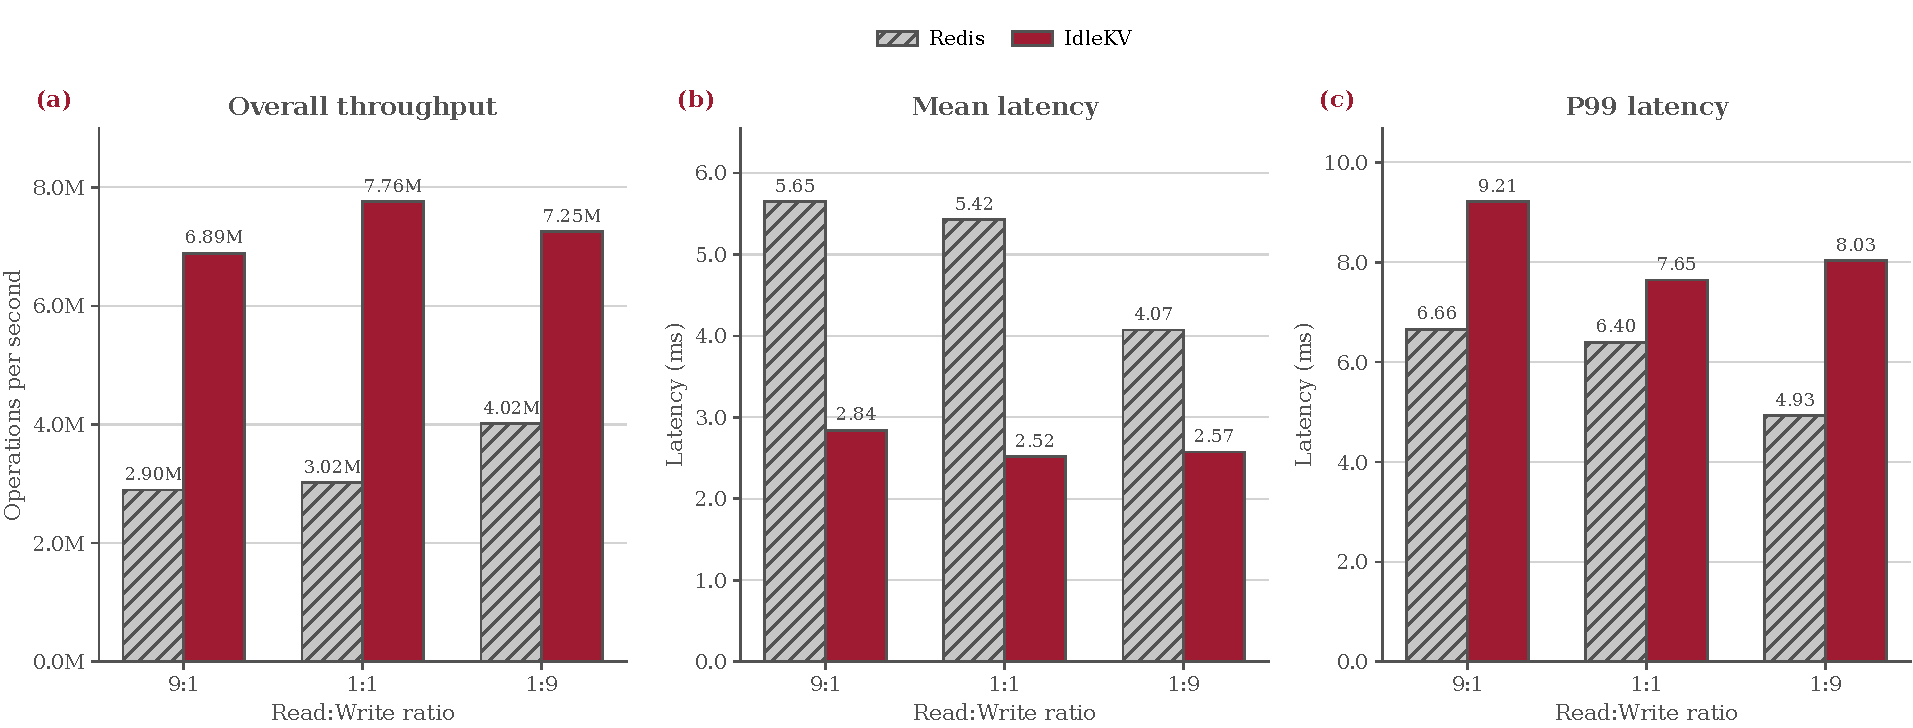
\includegraphics[width=1\textwidth]{get_set_benchmark/figures_pub/get_set_overview.pdf}
		\caption{Get/Set 工作负载总体对比}
		\label{fig:get-set-overview}
	\end{figure}

	图~\ref{fig:get-set-overview} 展示了两套系统在三组负载下的总体吞吐、平均延迟和 P99 延迟。可以看到，IdleKV 在三组负载中都显著领先于 Redis：在 \texttt{9:1}、\texttt{1:1} 和 \texttt{1:9} 三组负载下，总吞吐分别达到 6.89M、7.76M 和 7.25M ops/sec，而 Redis 分别为 2.90M、3.02M 和 4.02M ops/sec，对应吞吐提升为 2.38 倍、2.57 倍和 1.81 倍。平均延迟方面，IdleKV 分别为 2.84\,ms、2.52\,ms 和 2.57\,ms，均明显低于 Redis 的 5.65\,ms、5.42\,ms 和 4.07\,ms，说明系统在主路径上的请求处理效率得到了稳定改善。

	这一结果首先来自 Shared-Nothing 多线程架构对多核 CPU 的有效利用。Redis 的核心命令路径仍然主要由单线程串行推进，因此即使 \texttt{GET} 与 \texttt{SET} 本身足够轻量，总吞吐仍受限于单核执行能力。相比之下，IdleKV 将 key 按哈希分发到不同 shard，每个 shard 在独立线程中推进请求处理、事务注册与数据访问，从而把原本集中在单线程上的请求流分散到多个执行上下文中。对于本实验中的高并发 pipelined 负载，这种分片并行能够持续压缩队列等待时间，并把更多 CPU 周期用于实际命令执行，因此整体吞吐提升较为明显。

	不过，图~\ref{fig:get-set-overview} 也表明当前实现的尾延迟控制仍有改进空间。尽管 IdleKV 的平均延迟明显优于 Redis，但其 P99 延迟在三组负载下分别为 9.21\,ms、7.65\,ms 和 8.03\,ms，均高于 Redis 的 6.66\,ms、6.40\,ms 和 4.93\,ms。这说明 IdleKV 已经显著优化了大多数请求的常规执行路径，但少量请求仍可能受到 shard 队列排队、Fiber 调度、事务注册以及批量发送策略的影响，从而在尾部产生额外抖动。换言之，当前系统已经在吞吐与平均响应时间上建立明显优势，但在尾延迟稳定性方面仍需继续优化。

	\subsubsection{ZSet}
	本小节的实验数据仍在整理中，后续将补充 \texttt{ZADD}、\texttt{ZREM}、\texttt{ZRANGE} 等典型工作负载下的吞吐、平均延迟与尾延迟结果，并与 Redis 做进一步对比分析。

	\subsubsection{结果讨论}
	从已经完成的 \texttt{GET}/\texttt{SET} 实验来看，IdleKV 当前最明确的优势体现在基础命令路径上。Shared-Nothing 分片、多线程事件循环以及连接内批量处理共同降低了单位请求的调度摊销，使系统在单机多核环境下能够稳定获得高于 Redis 的总体吞吐，并在平均延迟上保持更优表现。这说明本文在运行时层面所采用的线程模型与分片执行策略是有效的。

	与此同时，实验也暴露出当前实现的若干工程短板。首先，系统虽然在平均路径上表现良好，但 P99 延迟仍弱于 Redis，表明尾延迟控制、调度公平性与批量发送策略仍需继续打磨。其次，\texttt{MULTI/EXEC} 等更完整的 Redis 事务语义尚未实现，Hash、Set、List 等对象类型的覆盖度也有限，这意味着当前原型更适合作为体系结构与数据结构设计验证平台，而非直接替代工程上成熟的 Redis。最后，有序索引路径的性能优势还需要结合后续 ZSet 实验进一步验证，尤其是 \texttt{ZRANGE} 深翻页、\texttt{ZADD} 更新和双索引维护成本等方面，仍有待通过系统化测试给出更完整的结论。

	\section{总结与展望}
	\subsection{工作总结}
	本文完成了一个面向 Redis 兼容语义的主内存键值数据库原型。系统在运行时层面构建了基于 Boost.Asio 与 Boost.Fiber 的多线程事件驱动框架，在执行层面实现了 Shared-Nothing 分片架构和基于 VLL 的事务注册机制，在数据结构层面实现了基于 ART 的 ZSet 双索引结构，并通过 Get/Set 与 ZSet 两类实验验证了整体设计的有效性。综合来看，IdleKV 已经具备了较清晰的模块边界、可运行的事务调度路径和后续继续扩展的工程基础。

	\subsection{不足分析}
	当前系统仍存在若干明显不足。首先，事务框架已经支持单命令事务型操作和跨 shard 的多 key 命令，但 Redis 的 \texttt{MULTI/EXEC} 原子多命令事务尚未实现；其次，命令覆盖范围仍然有限，Hash、List、Set 等对象类型还未形成完整能力；再次，\texttt{TxnQueue}、锁表和 ART/ZSet 等关键路径虽然已可工作，但还缺少在更复杂负载和更大规模数据集上的系统化验证。

	\subsection{后续工作}
	后续工作可从两个方向继续推进。第一，继续扩展事务层，补齐 \texttt{MULTI/EXEC} 等原子多命令语义，并研究更完善的阻塞队列、公平性和冲突处理策略。第二，继续增强 ART 与容器对象实现，补充更多真实业务负载下的性能测试与工程验证。

	\newpage
	\phantomsection
	\addcontentsline{toc}{section}{参考文献}
	\begingroup
	\setlength{\bibsep}{0pt}
	\setlength{\parskip}{0pt}
	\setlength{\itemsep}{0pt}
	\setlength{\parsep}{0pt}
	\setlength{\topsep}{0pt}
	\setlength{\partopsep}{0pt}
	\begin{spacing}{1.5}
	\bibliographystyle{gbt7714-numerical}
	\bibliography{references}
	\end{spacing}
	\endgroup



\end{spacing}

\end{document}
